\documentclass[a4paper,11pt,oneside]{book}

\usepackage[english]{babel}
\usepackage[showframe=false]{geometry}
\usepackage[usenames,dvipsnames]{xcolor}
\usepackage[utf8]{inputenc}
\usepackage[T1]{fontenc}
\usepackage{changepage}
\usepackage[]{algorithm2e}
\usepackage{amssymb}
\usepackage{amsmath}
\usepackage{graphicx}
\usepackage{listings}
\usepackage{verbatimbox}
\usepackage{ulem}
\usepackage{fancyvrb}
\usepackage{float}
\usepackage{hyperref}
\usepackage[parfill]{parskip}
\usepackage{tikz}
\usepackage{pdflscape}
\usepackage{minted}
\usepackage{titlesec}
\usepackage{titleps}
\usepackage{lastpage}
\usepackage{fancyhdr}
\usepackage{etoolbox}
%Following overwrites the page style for chapters
\patchcmd{\chapter}{\thispagestyle{plain}}{\thispagestyle{ruledChapter}}{}{}

%New page style for chapters
\newpagestyle{ruledChapter}{
	\setfoot{}{\thepage\ of \pageref{LastPage}}{}
	\footrule
	\renewcommand\makefootrule{\color{black}\rule[\baselineskip]{\linewidth}{0.4pt}}
}
%New page style for rest
\newpagestyle{ruled}{
	\sethead{\raggedright \chaptername\ \thechapter :\ \chaptertitle}{}{}
	\headrule
	\setfoot{}{\thepage\ of \pageref{LastPage}}{}
	\footrule
	\renewcommand\makeheadrule{\color{black}\rule[-.3\baselineskip]{\linewidth}{0.4pt}}
	\renewcommand\makefootrule{\color{black}\rule[\baselineskip]{\linewidth}{0.4pt}}
}

\expandafter\def\csname PY@tok@err\endcsname{}
\newcommand{\HRule}{\rule{\linewidth}{0.5mm}}
\newcommand{\specialcell}[2][c]{%
  \begin{tabular}[#1]{@{}c@{}}#2\end{tabular}}

\addtocontents{toc}{\protect\thispagestyle{empty}}

\title{}
\author{}
\date{} 

\begin{document}
\begin{titlepage}
\begin{center}

%-----------------------------------------------------------------
%							FRONTPAGE
%-----------------------------------------------------------------
\thispagestyle{empty}

\includegraphics[width=0.55\textwidth]{logo.pdf}\\[1cm]    
\textsc{\Large DM818 Assignment 1}\\[0.5cm]

% Title
\begin{Huge}
\textbf{Matrix Multiplication}
\end{Huge}

\vspace{4cm}

% Author and supervisor
\begin{minipage}{1\textwidth}
\begin{center}
\emph{}\\

Dan \textsc{Sebastian Thrane}\\
\verb!<dathr12@student.sdu.dk>!\\

Lars \textsc{Thomasen}\\
\verb!<latho12@student.sdu.dk>!\\

\end{center}
\end{minipage}
\begin{minipage}{0.4\textwidth}
\end{minipage}

\vfill
\begin{tabular}{ll}
    Aligned SSE: yes \\
    Unaligned SSE: no \\
\end{tabular}
\vfill

% Bottom of the page
{\large Fall 2015}\\

\end{center}
\end{titlepage}

%-----------------------------------------------------------------
%							   TOC
%-----------------------------------------------------------------
\renewcommand{\contentsname}{Table of Contents}
\tableofcontents
\thispagestyle{empty}

%-----------------------------------------------------------------
%						  ACTUAL REPORT
%-----------------------------------------------------------------
\pagestyle{ruled}
\chapter{Introduction}
\setcounter{section}{1}

This report covers the task of optimizing matrix multiplication on a single
core. For this task access to the NERSC cluster has been supplied, thus majority
of the performance tweaking was been focused for this. Code for running on the
SDU Imada terminal room has also been developed, however values are not tweaked
as well there.

\section{Work Load}

This assignment has been done in a group of two, following pair programming
principles. Thus the work load has been evenly divided, majority of the work
load being converting theoretical theories into actual code and doing things
correctly.

\chapter{Optimizations}
% The optimizations used or attempted
% The results of those optimizations
\section{Overview}

The basis of our algorithm is a blocked approach based on a proposed algorithm
from Goto. % TODO Proper reference 

The overall plan for this algorithm consists of three phases:

% TODO Make sure that the following claims are correct. This section is meant to
% be a somewhat informal overview of the algorithm.

\begin{enumerate}
  \item Split the input matrices into slivers. Matrix A will be split into 
  slivers of columns, matrix B will be split into slivers of rows. A is split
  into slivers of columns, and B into rows, because of the access pattern that
  will be used during the actual multiplication phase, and as such improve the
  data access pattern, and minimize the number of movements between memory
  layers.
  \item Split the matrices up into smaller blocks, and begin packing the data.
  The smaller blocks are chosen such that they may reside inside of a single
  memory layer. The data is packed such that it will be placed sequentially in
  memory with accordance to how the data will be accessed by the program. 
  The data should be packed shortly before use, such that it can stay as close 
  to the CPU as possible.
  \item Perform efficient matrix multiplication between these small blocks.
\end{enumerate}

% TODO Talk about sizes of matrices

The following sections will go into details of how these phases were
implemented, and how the results observed guided further optimizations.

\subsection{Efficient Inner Matrix Multiplication}

It is the job of the other phases to ensure that data is laid out in memory,
such that movement between memory layers are minimized. It is the job of this
phase to as efficiently as possible do raw number crunching.

The Intel architecture available on both Hopper, and on the IMADA machines used
for development, both provide a set of SSE instructions. These instructions are
SIMD instructions. Single instruction, multiple data (SIMD) is a form of
parallelism with multiple processing elements that perform the same operation on
multiple data simultaneously. This means that we can multiply several numbers
with each other at the same time. 

By using SIMD instructions, we are able to cut the K iterations in half by doing
two iterations at the same time with no additional cost. As a result we saw a
significant performance improvement. %true? Do we have any before-after numbers?

However to using SSE instructions efficiently requires the data to be properly
aligned at a 16-byte offset. % TODO reference to manual 
Since we do not have control of how the input data is stored, this will require 
copying the data, and assure that the data is copied to start at a properly 
aligned address. 

The SSE instructions will always work on two double-precision floating point
numbers. This provides us with an edge-case when the inner loop works on
matrices with dimensions that aren't a multiple of two. This problem became even
more important when loop unrolling was performed to further optimize
performance. We simply dealt with the problem by padding the matrices.

% TODO Do we put any code here?

\subsection{Preparing the Data}

In order to improve data locality, and take advantage of loading SSE
instructions, data had to be re-arranged. This required new auxiliary arrays for
the packed data, aligning it for 16 bytes. Since this data would have to be
loaded regardless, then we won't incur any additional movement between the 
memory layers. % TODO Not trivial, not sure this is enough, what about 
% overhead from writing?

We first pack the entire B matrix, and then pack the A matrix in slivers of size
$mc$. The order of this packaging ensures that the relevant $mc$ rows of the A
matrix is always in memory along with most, if not all, of the B matrix too. By
packing slivers of the A matrix we are able to increase the block size in
general and still keep it all in memory. The idea behind this is that when we
load in the next sliver of A, the least recently used data will be the old A
matrix. %TODO: I need to rewrite this section.

\subsection{Loop Unrolling}

% TODO: I need to read up a slight bit on exactly how this works, but the gist
% of it is correct. (What is the difference between hardware pipelning and
% software pipelining exactly?).

In order to exploit pipelining, loop unrolling has been performed in the inner-
most matrix multiplication. By loop unrolling the actual multiplication of the
elements, the hardware is able to do several computations at once, before having
to wait for the multiplication to finish and continuing the loop.

% Insert code example here?

%Padding:

In order to perform loop unrolling, padding was initially used such that fringe
cases would not cause the program to access data outside of the arrays. This
padding was done by simply putting the value 0 into the additional elements
accessed, as this would not change the correctness of the matrix multiplication.

This padding resulted in performance dips for matrix sizes which did not fit
into a multiplicative of the unrolled size. This behaviour is clearly seen in
the figure below. The explanation for this lies in the added calculations of the
zeroes, along with using an auxiliary array for the result matrix.

The auxiliary array was necessary as padding the result matrix was infeasible
when writing to values outside its array. This writing to a temp array and
moving only the relevant entries was the best solution we could come up with.

\begin{figure}
  \centering
  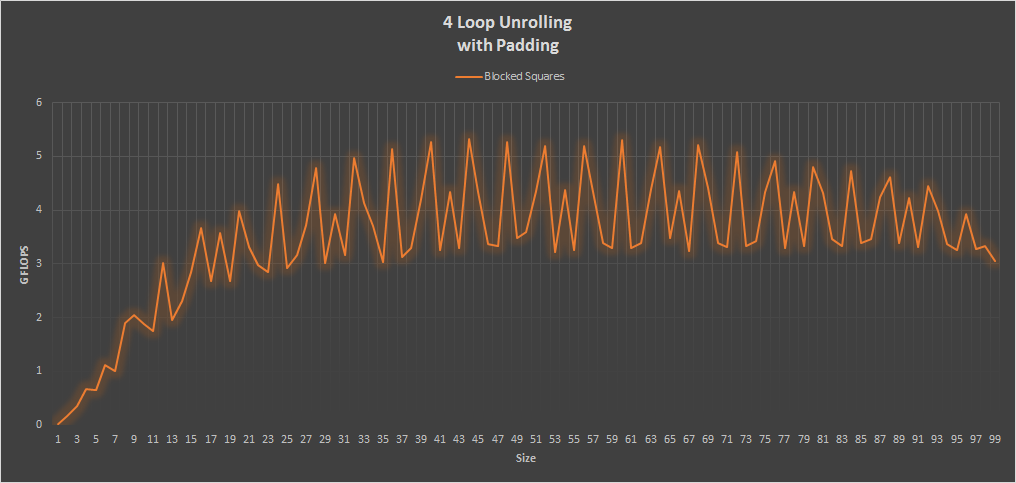
\includegraphics[width=0.9\linewidth]{graph-blocked-padding.png}
  \caption{Unrolling the access to the B matrix with 4, using padding to handle 
           fringe cases.}
  \centering
  \label{fig:sub1}
\end{figure}

This solution was improved upon by doing an early check of the actual block
size, and then calling the method best fitted for that block size, such that
loop unrolling could be maximized.

\subsection{Fringe Cases and Padding}

The padding however introduced yet another problem. When reaching certain fringe
cases, these padded entries would result in entries into the $C$ matrix which
would be out of bounds.

As we saw in the loop unrolling section, we use different procedures depending
on which case we are dealing with. We used this to avoid adding padding, when we
knew that it wouldn't ever be required. This obviously means that we won't have
to deal with going out of bounds in this special case, since we know that it
cannot happen, due to no padding being added. In the case that padding may be
added, we however had to deal with this problem. The two most simple approaches 
to this are:

\begin{enumerate}
  \item Run-time checks to avoid going out of bounds
  \item Use an auxiliary matrix, which also contains padding, and copy this to 
        the real output matrix
\end{enumerate}

Approach 1 may be the most traditional way of dealing with out-of-bounds
behavior, when writing code that isn't performance critical. However this
approach leads to a large amount of branching. Which the loop unrolling
optimization also showed, leads to a significant performance loss.

Approach 2 has a small amount of overhead involved in copying the data from the
auxiliary matrix into the output matrix, however our observations showed that
this was still better than going with approach 1.

% TODO Did we ever try using approach 1? Would be nice with some numbers to 
% show that we actually did the right thing

\subsection{Choosing Block Sizes}


\chapter{Performance}

% How the same kernel performs on a different hardware platform (and a small
% discussion of that) TODO: Need to test this, Hooper VS Imada, and how the
% different architectures are (since this is the primary reason for variation).

\section{Hopper}
\subsection{Graphs}

% A figure fhat shows the performance similar than the figure above, but using
% all matrix sizes 2, 3, 4, ..., 769 for a single processor core of NERSC Hopper
% cluster (y-axis should say percentage of peak performace).

Below is a graph comparing the different algorithms. The Naive, Transposed, and BLAS algorithms are the one from the assignment. The Blocked algorithm is the implementation following the precious sections. All have been run on hopper, scheduled with a single node.

\begin{figure}[H]
  \centering
  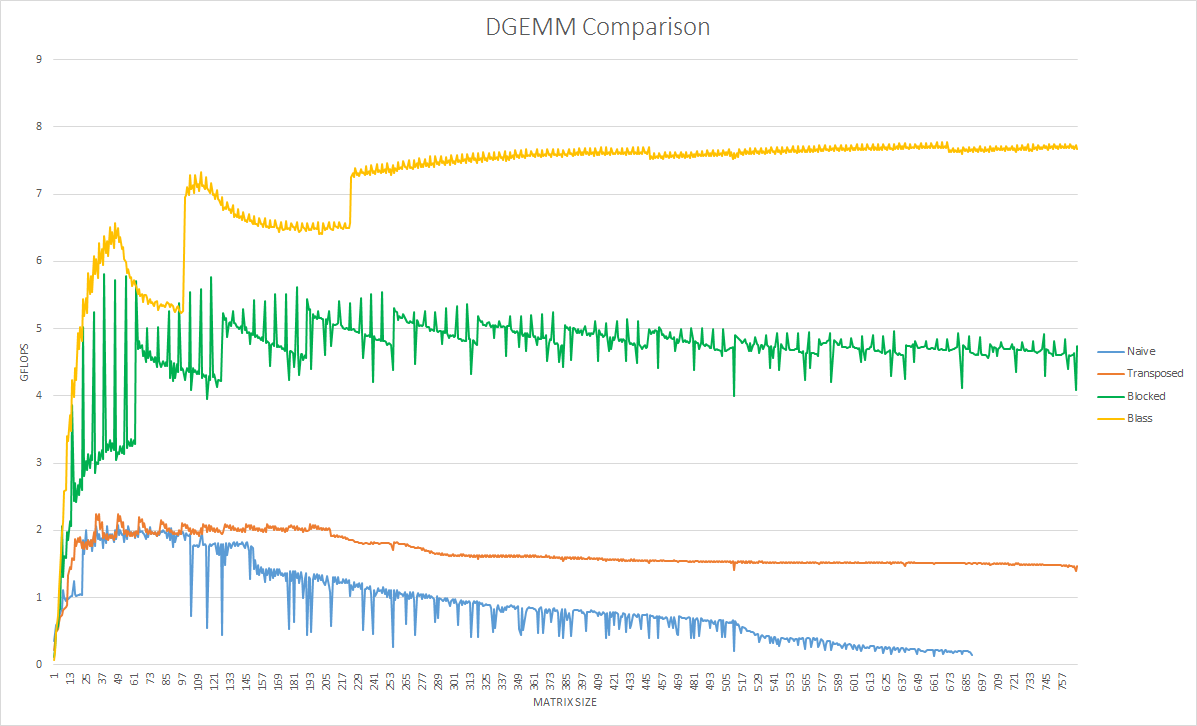
\includegraphics[width=0.9\linewidth]{comparison-graph.png}
  \caption{Comparing different algorithms with our implementation. The Blocked is the performance we arrived at.}
  \centering
  \label{fig:sub1}
\end{figure}

\subsection{Odd Behaviours}
% The reason for any odd behavior (e.g., dips) in performance.
The constant variation in the blocked algorithm comes from the different matrix sizes. The peaks are whenever the matrix fringe cases are non-existent. Thus the matrix has $Size%BLOCK_SIZE == 0$. % Er ikke engang helt sikker på dette er den eneste grund.

\subsection{Peak Performance}
% Explain how you determined the peak performace, and again, the y-axis should
% say percentage of peak performance.

\begin{figure}[H]
  \centering
  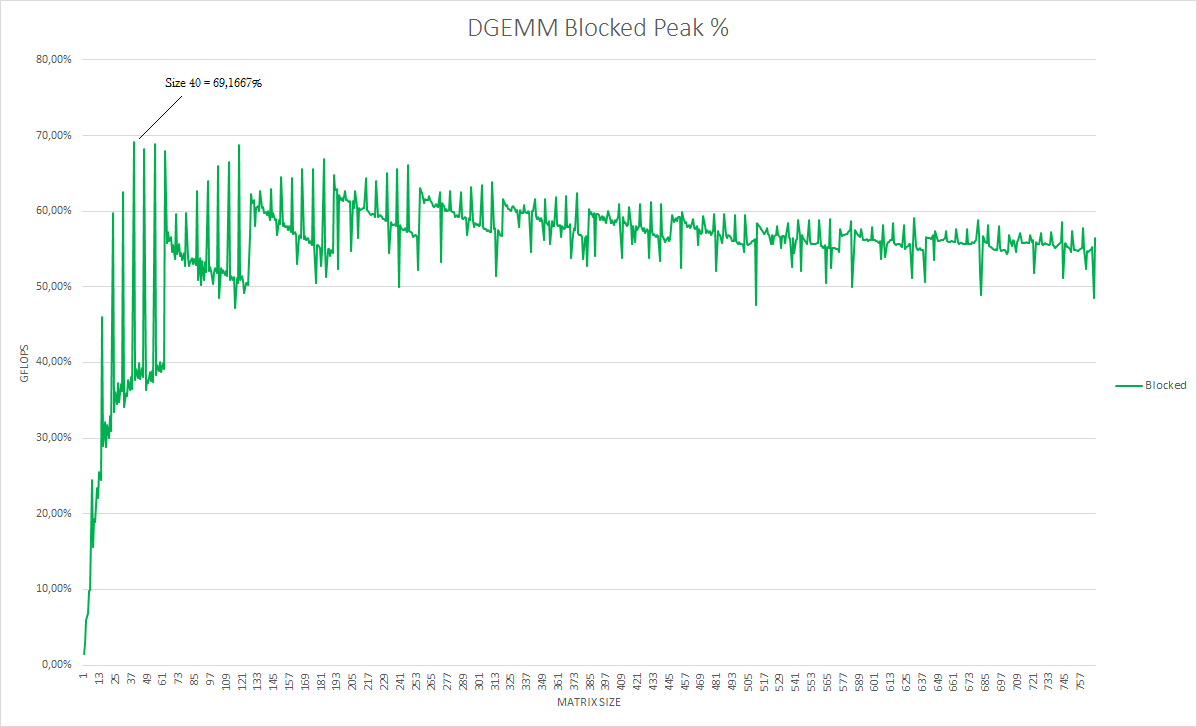
\includegraphics[width=0.9\linewidth]{peak-graph.png}
  \caption{Comparing different algorithms with our implementation. The Blocked is the performance we arrived at.}
  \centering
  \label{fig:sub1}
\end{figure}

The average peak-performance across sizes 2 to 769 is $55,235%$.

\section{IMADA Machines}
\subsection{Graphs}
% A figure fhat shows the performace similar than the figure above, but using
% all matrix sizes 2, 3, 4, ..., 769 for a single processor of another system of
% your choice (using the same kernel).

Below is a graph like the previous, but instead run on the Imada terminal room.

\begin{figure}[H]
  \centering
  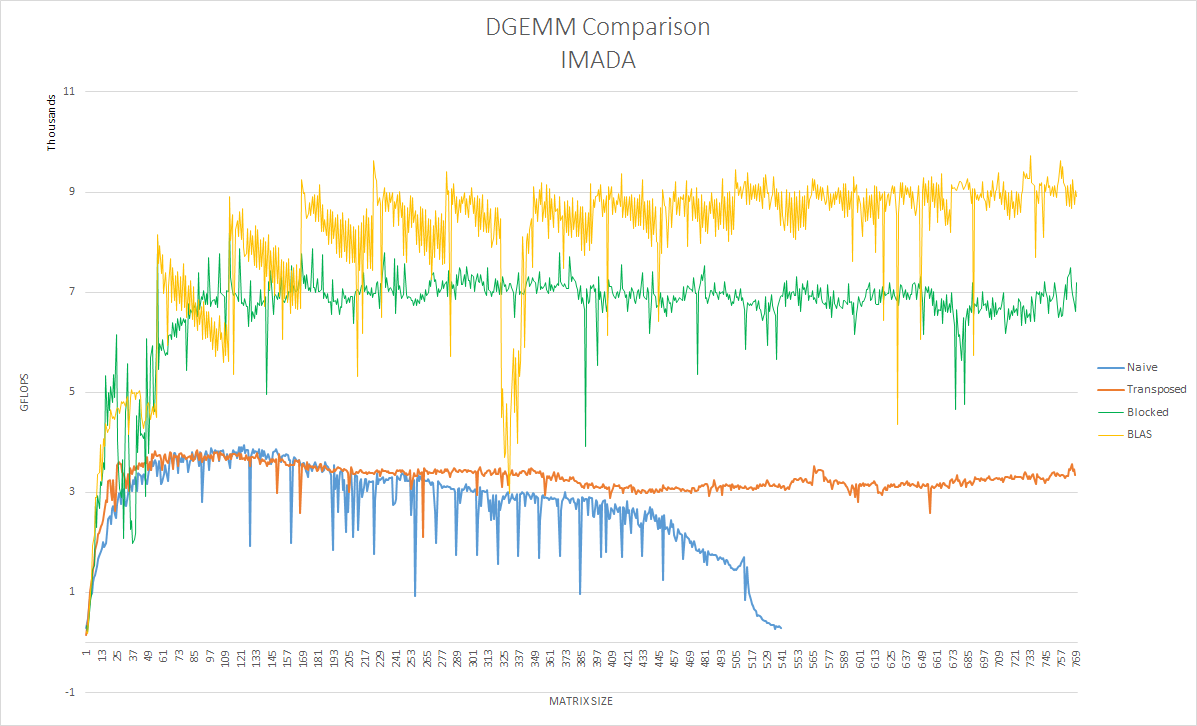
\includegraphics[width=0.9\linewidth]{comparison-graph-imada.png}
  \caption{Comparing different algorithms with our implementation. The Blocked is the performance we arrived at.}
  \centering
  \label{fig:sub1}
\end{figure}


\chapter{Conclusion}
% A short recap of what we achieved and the results.


%-----------------------------------------------------------------
%						     APPENDIX
%-----------------------------------------------------------------
%\newpage
%\newgeometry{left=2.5cm,right=2.5cm}
%\chapter{Appendix}
%\section{Source code}

\end{document}
